\section{Results}
\label{sec:results}

We organise the results around three questions.
\secref{sec:results:ppl} asks which interventions preserve fluency and are
therefore behaviourally interpretable. \secref{sec:results:dat} reports
\dat under those interventions, broken down by model and decoder.
\secref{sec:results:96trio} documents the gibberish-driven \dat-inflation
artifact. \secref{sec:results:geom} reports per-layer concept-association
geometry. \secref{sec:results:reconcile} reconciles geometry and behaviour.

\subsection{Perplexity Sanity Check: Which Interventions Are Usable?}
\label{sec:results:ppl}

\tabref{tab:ppl} summarises perplexity on a $113$-token calibration text.
Across all three models, only \nomean (\rmsnorm-equivalent) preserves
fluency: whole-model \nomean adds $3\%\!-\!35\%$ perplexity, and
layer-targeted \nomean is essentially free ($\le 5\%$). \noaffine breaks
the model by $10^{2}\!-\!10^{3}\times$. \weakened with $\alpha\le 0.5$ and
\identityln are catastrophic ($10^{3}\!-\!10^{5}\times$ or NaN). We
therefore restrict the behavioural analysis to the comparison
$\stockln$ vs.\ $\nomean\times\{\tgtall,\tgtearly,\tgtmid,\tgtlate\}$ and
report broken interventions only for completeness.

\begin{table}[t]
\centering
\caption{Perplexity on a 113-token calibration text. Only \nomean
preserves fluency; all stronger ablations break the model. ``inf'' = NaN
loss; ``--'' = not applicable.}
\label{tab:ppl}
\begin{tabular}{@{}lllrl@{}}
\toprule
\textbf{Model} & \textbf{Recipe} & \textbf{Target} & \textbf{PPL} & \textbf{Verdict} \\
\midrule
\gptsmall  & \stockln    & --     & \textbf{24.4}        & baseline \\
\gptsmall  & \nomean     & \tgtall    & 27.3                 & $+12\%$, usable \\
\gptsmall  & \nomean     & early/mid/late & $24\!-\!26$      & usable \\
\gptsmall  & \noaffine   & \tgtall    & 3{,}041              & broken \\
\gptsmall  & \weakened   & \tgtall ($\alpha{=}0.75$) & 9{,}130 & broken \\
\gptsmall  & \weakened/\identityln & \tgtall   & inf                  & broken \\
\midrule
\pythia    & \stockln    & --     & \textbf{15.3}        & baseline \\
\pythia    & \nomean     & \tgtall    & 15.8                 & $+3\%$, usable \\
\pythia    & \nomean     & early/mid/late & $15.1\!-\!15.9$  & usable \\
\pythia    & \noaffine   & \tgtall    & 64                   & broken \\
\pythia    & \weakened   & \tgtall    & $1{,}500\!-\!150{,}000$ & broken \\
\pythia    & \identityln & \tgtall    & 4{,}862              & broken \\
\midrule
\gptmedium & \stockln    & --     & \textbf{16.7}        & baseline \\
\gptmedium & \nomean     & \tgtall    & 22.6                 & $+35\%$, usable \\
\gptmedium & \nomean     & early/mid/late & $16.7\!-\!18.9$  & usable \\
\gptmedium & \weakened/\identityln & \tgtall   & inf       & broken \\
\bottomrule
\end{tabular}
\end{table}

\subsection{DAT Scores Under Fluency-Preserving Interventions}
\label{sec:results:dat}

\Figref{fig:main_dat} shows the full \dat panel, faceted by (model, decoder),
with stock as a horizontal reference. The headline pattern is summarised
by tables \ref{tab:dat-gpt2-topp}--\ref{tab:dat-gpt2-hight}.

\begin{figure}[t]
\centering
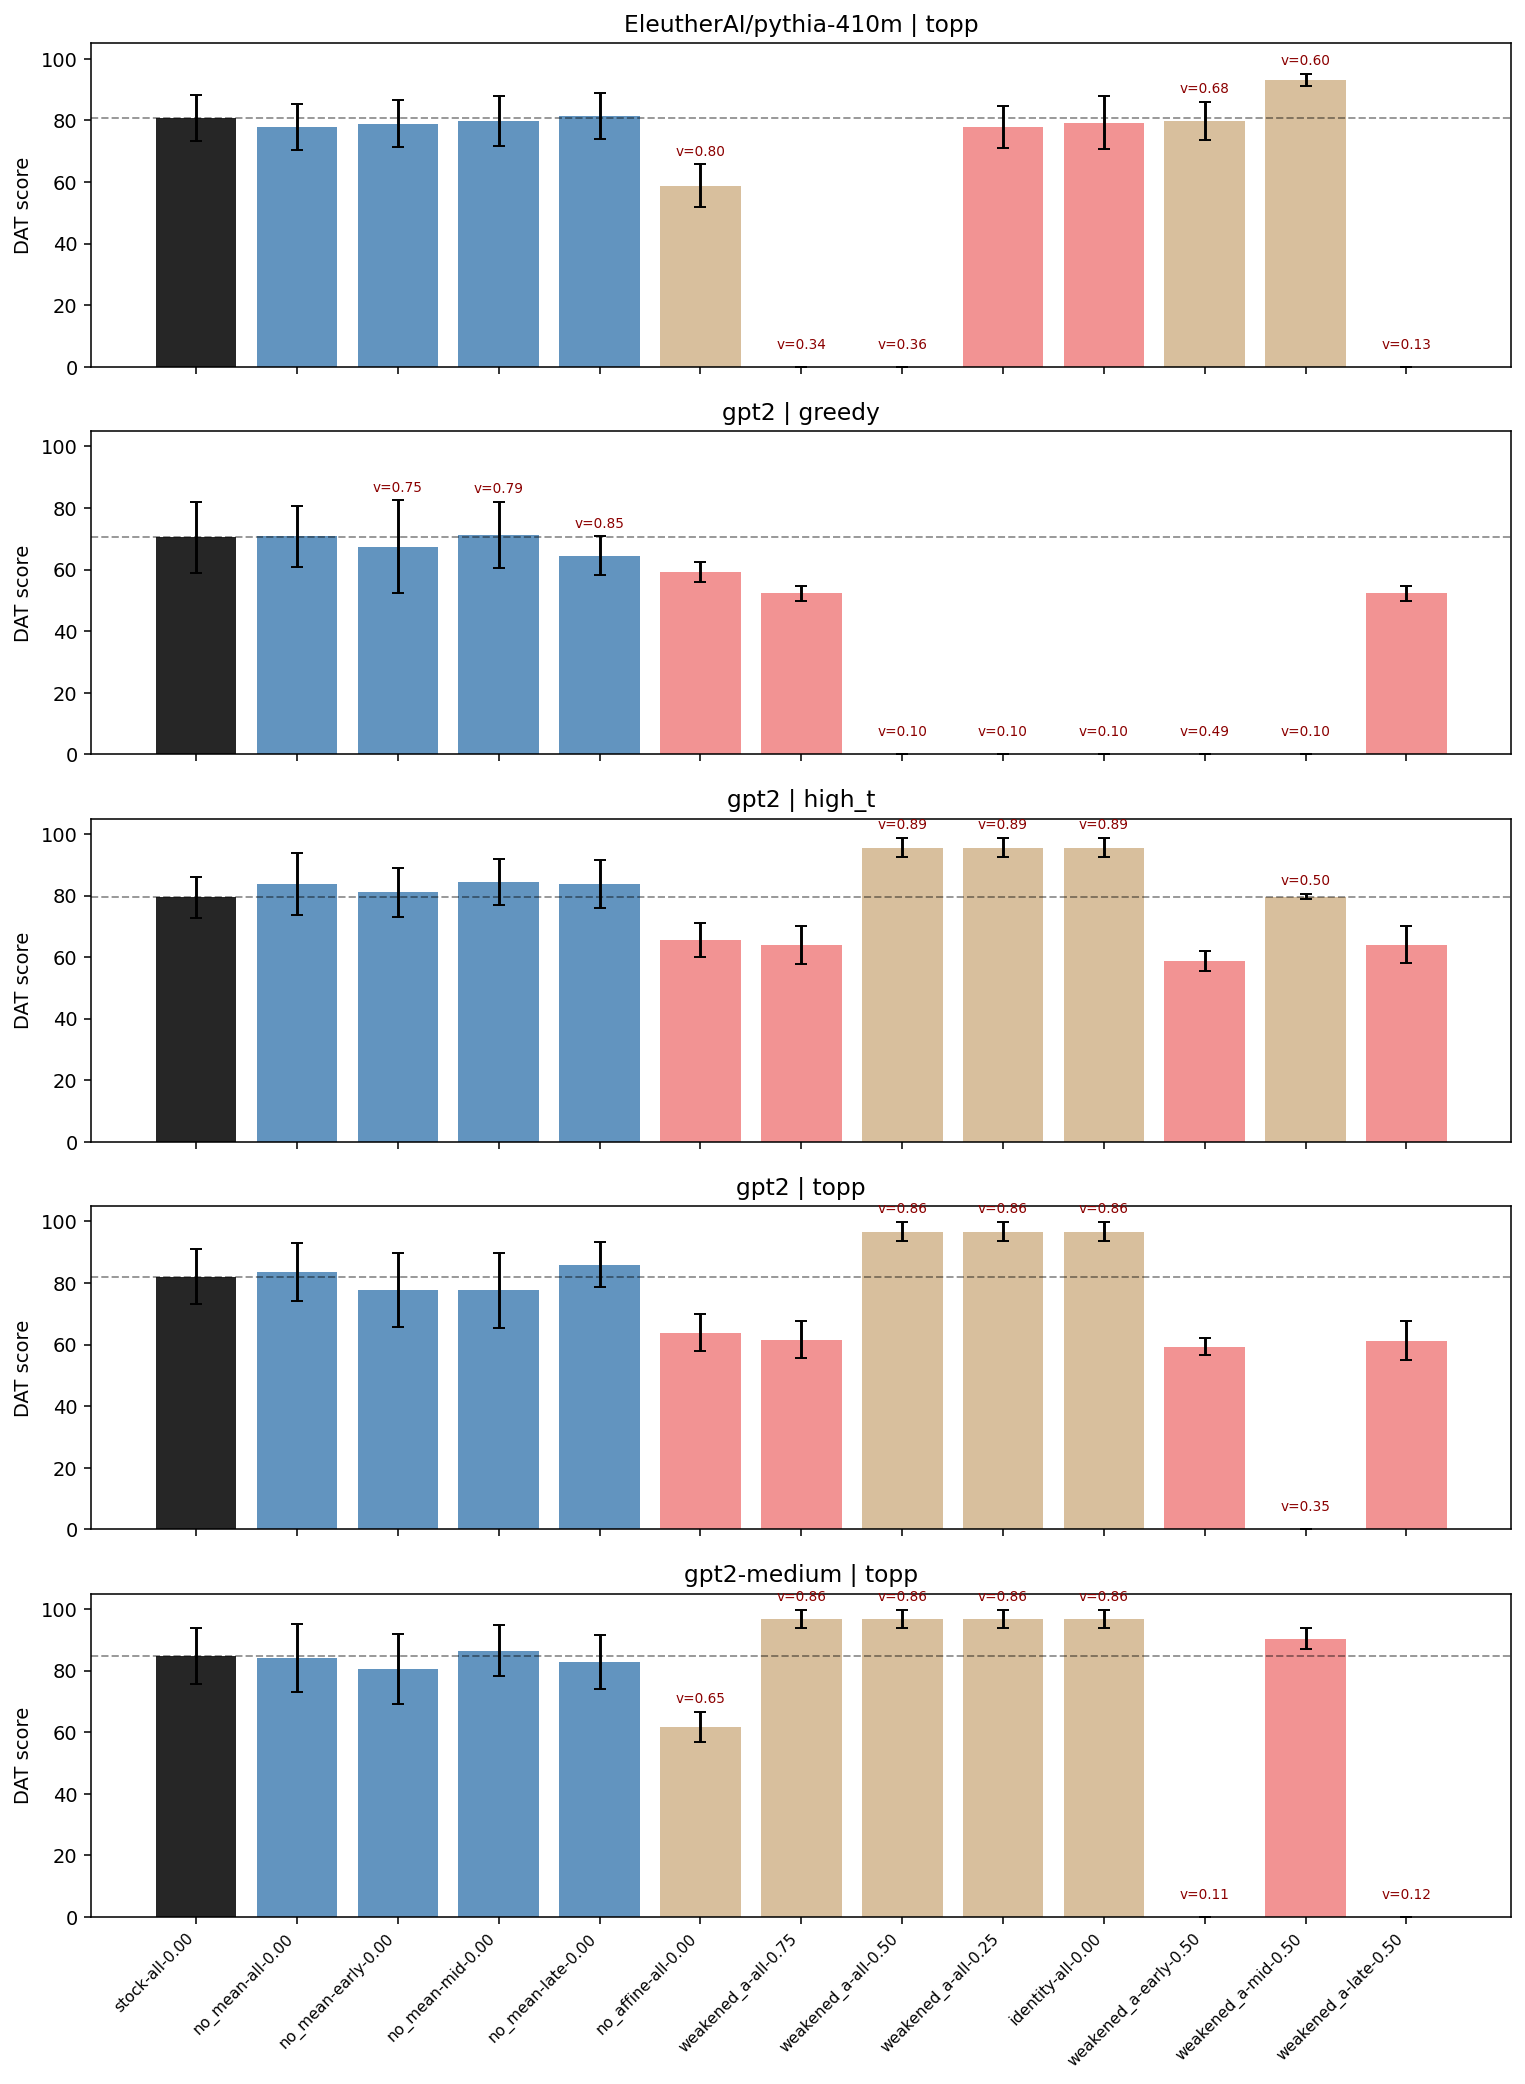
\includegraphics[width=0.95\linewidth]{figures/main_dat_panel.png}
\caption{\dat under all interventions, faceted by model and decoder.
Validity rate is overlaid as a thin line. Only \nomean (orange/blue family)
preserves validity $\ge 0.9$. The $T{=}1.2$ panel for \gptsmall (rightmost
column) is the only panel where \emph{all four} \nomean targets push \dat
above stock.}
\label{fig:main_dat}
\end{figure}

\begin{table}[t]
\centering
\caption{\gptsmall + \topp ($T{=}0.7$, top-$p{=}0.9$), $n{=}20$. \dat values
are mean$\pm$SD. $\Delta$ is mean shift versus \stockln; $d$ is Cohen's
$d$. None of the cells survive Bonferroni at $\alpha{=}0.003$.}
\label{tab:dat-gpt2-topp}
\begin{tabular}{@{}lcccrr@{}}
\toprule
\textbf{Intervention} & \textbf{\dat} & \textbf{Validity} & $\Delta$ & $d$ & $p$ \\
\midrule
\stockln          & \textbf{82.13$\pm$9.06}  & 1.00 & --    & --    & -- \\
\nomean (\tgtall)  & 83.58$\pm$9.34          & 1.00 & $+1.45$ & $+0.15$ & 0.47 \\
\nomean (\tgtearly)& 77.86$\pm$11.97         & 1.00 & $-4.27$ & $-0.39$ & 0.27 \\
\nomean (\tgtmid)  & 77.65$\pm$12.13         & 1.00 & $-4.48$ & $-0.41$ & 0.32 \\
\nomean (\tgtlate) & \textbf{86.02$\pm$7.21} & 1.00 & $\mathbf{+3.89}$ & $\mathbf{+0.46}$ & 0.23 \\
\bottomrule
\end{tabular}
\end{table}

\begin{table}[t]
\centering
\caption{\gptsmall + \greedy, $n{=}20$. Note that \nomean (\tgtall) lifts
validity from $0.73$ to $0.97$ without changing \dat: the model becomes
more parseable but no more diverse, ruling out a ``stock \gptsmall is bad
at format'' confound.}
\label{tab:dat-gpt2-greedy}
\begin{tabular}{@{}lcccrr@{}}
\toprule
\textbf{Intervention} & \textbf{\dat} & \textbf{Validity} & $\Delta$ & $d$ & $p$ \\
\midrule
\stockln           & 70.49$\pm$11.47 & 0.73 & --    & --    & -- \\
\nomean (\tgtall)   & 70.78$\pm$9.86  & \textbf{0.97} & $+0.29$ & $+0.03$ & 0.79 \\
\nomean (\tgtearly) & 67.48$\pm$14.97 & 0.75 & $-3.01$ & $-0.22$ & 0.66 \\
\nomean (\tgtmid)   & 71.15$\pm$10.79 & 0.79 & $+0.66$ & $+0.06$ & 0.94 \\
\nomean (\tgtlate)  & 64.48$\pm$6.26  & 0.85 & $-6.00$ & $-0.64$ & 0.10 \\
\bottomrule
\end{tabular}
\end{table}

\begin{table}[t]
\centering
\caption{\gptmedium + \topp, $n{=}20$. Direction of \dat shifts is
inconsistent across layer targets.}
\label{tab:dat-gptmedium-topp}
\begin{tabular}{@{}lcccrr@{}}
\toprule
\textbf{Intervention} & \textbf{\dat} & \textbf{Validity} & $\Delta$ & $d$ & $p$ \\
\midrule
\stockln           & \textbf{84.69$\pm$9.08} & 0.99 & --    & --    & -- \\
\nomean (\tgtall)   & 84.06$\pm$11.02 & 0.94 & $-0.63$ & $-0.06$ & 1.00 \\
\nomean (\tgtearly) & 80.55$\pm$11.24 & 0.97 & $-4.15$ & $-0.40$ & 0.27 \\
\nomean (\tgtmid)   & \textbf{86.51$\pm$8.32} & 0.98 & $\mathbf{+1.82}$ & $\mathbf{+0.20}$ & 0.60 \\
\nomean (\tgtlate)  & 82.85$\pm$8.84  & 1.00 & $-1.84$ & $-0.20$ & 0.52 \\
\bottomrule
\end{tabular}
\end{table}

\begin{table}[t]
\centering
\caption{\pythia + \topp, $n{=}20$.}
\label{tab:dat-pythia-topp}
\begin{tabular}{@{}lcccrr@{}}
\toprule
\textbf{Intervention} & \textbf{\dat} & \textbf{Validity} & $\Delta$ & $d$ & $p$ \\
\midrule
\stockln           & \textbf{80.93$\pm$7.47} & 1.00 & --    & --    & -- \\
\nomean (\tgtall)   & 77.86$\pm$7.54 & 1.00 & $-3.07$ & $-0.40$ & 0.21 \\
\nomean (\tgtearly) & 78.95$\pm$7.52 & 1.00 & $-1.98$ & $-0.26$ & 0.41 \\
\nomean (\tgtmid)   & 79.67$\pm$8.12 & 1.00 & $-1.26$ & $-0.16$ & 0.68 \\
\nomean (\tgtlate)  & 81.33$\pm$7.43 & 1.00 & $+0.40$ & $+0.05$ & 0.94 \\
\bottomrule
\end{tabular}
\end{table}

\begin{table}[t]
\centering
\caption{\gptsmall + \hight ($T{=}1.2$, top-$p{=}0.95$), $n{=}15$. \emph{All
four} \nomean targets push \dat positive, with $d{>}{+}0.2$ across the
board --- the only panel where this happens.}
\label{tab:dat-gpt2-hight}
\begin{tabular}{@{}lcccrr@{}}
\toprule
\textbf{Intervention} & \textbf{\dat} & \textbf{Validity} & $\Delta$ & $d$ & $p$ \\
\midrule
\stockln           & \textbf{79.39$\pm$6.70} & 1.00 & --    & --    & -- \\
\nomean (\tgtall)   & \textbf{83.70$\pm$9.97} & 0.99 & $\mathbf{+4.31}$ & $\mathbf{+0.49}$ & 0.62 \\
\nomean (\tgtearly) & 81.07$\pm$7.92 & 1.00 & $+1.68$ & $+0.22$ & 0.72 \\
\nomean (\tgtmid)   & \textbf{84.46$\pm$7.47} & 1.00 & $\mathbf{+5.07}$ & $\mathbf{+0.69}$ & 0.15 \\
\nomean (\tgtlate)  & \textbf{83.84$\pm$7.76} & 1.00 & $\mathbf{+4.45}$ & $\mathbf{+0.59}$ & 0.21 \\
\bottomrule
\end{tabular}
\end{table}

\para{Cross-panel summary.}
Across the $18$ fluency-preserving cells, the largest absolute \dat shift
is $|6.0|$ (\gptsmall \greedy \tgtlate, negative) and no cell crosses
Bonferroni at $\alpha{=}0.003$ (smallest $p{=}0.10$). The notable pattern
is the high-$T$ panel for \gptsmall: all four \nomean targets push \dat
in the same positive direction by $+1.7$ to $+5.1$ points with all
$d{>}{+}0.2$ --- the only panel where this happens. Under low-$T$ or
\greedy, no model shows a consistent direction. We treat the unanimous
high-$T$ direction as suggestive but underpowered, not a confirmed effect.

\subsection{The Artifactual ``96.73 Trio''}
\label{sec:results:96trio}

For both \gptsmall and \gptmedium under \topp, three completely-broken
interventions (\weakened with $\alpha{=}0.5$, \weakened with $\alpha{=}0.25$,
and \identityln) collapse to the \emph{same} \dat mean of $96.73\pm 2.97$
with validity $0.86$ and infinite perplexity. Inspecting the generated
words shows the model emits $\sim\!17$ \glove-valid but semantically random
tokens such as ``stellarnazi'', ``metallicmerce'', ``disruptingrived''.
These are out-of-distribution junk whose \glove embeddings are effectively
random and therefore far apart in cosine. \Figref{fig:dat-vs-validity}
makes this Pareto-clear: the highest \dat scores in our experiment all
correspond to the lowest validity. This is a clean failure mode of \dat
when applied to broken models and motivates our use of validity rate as a
co-equal sanity check.

\begin{figure}[t]
\centering
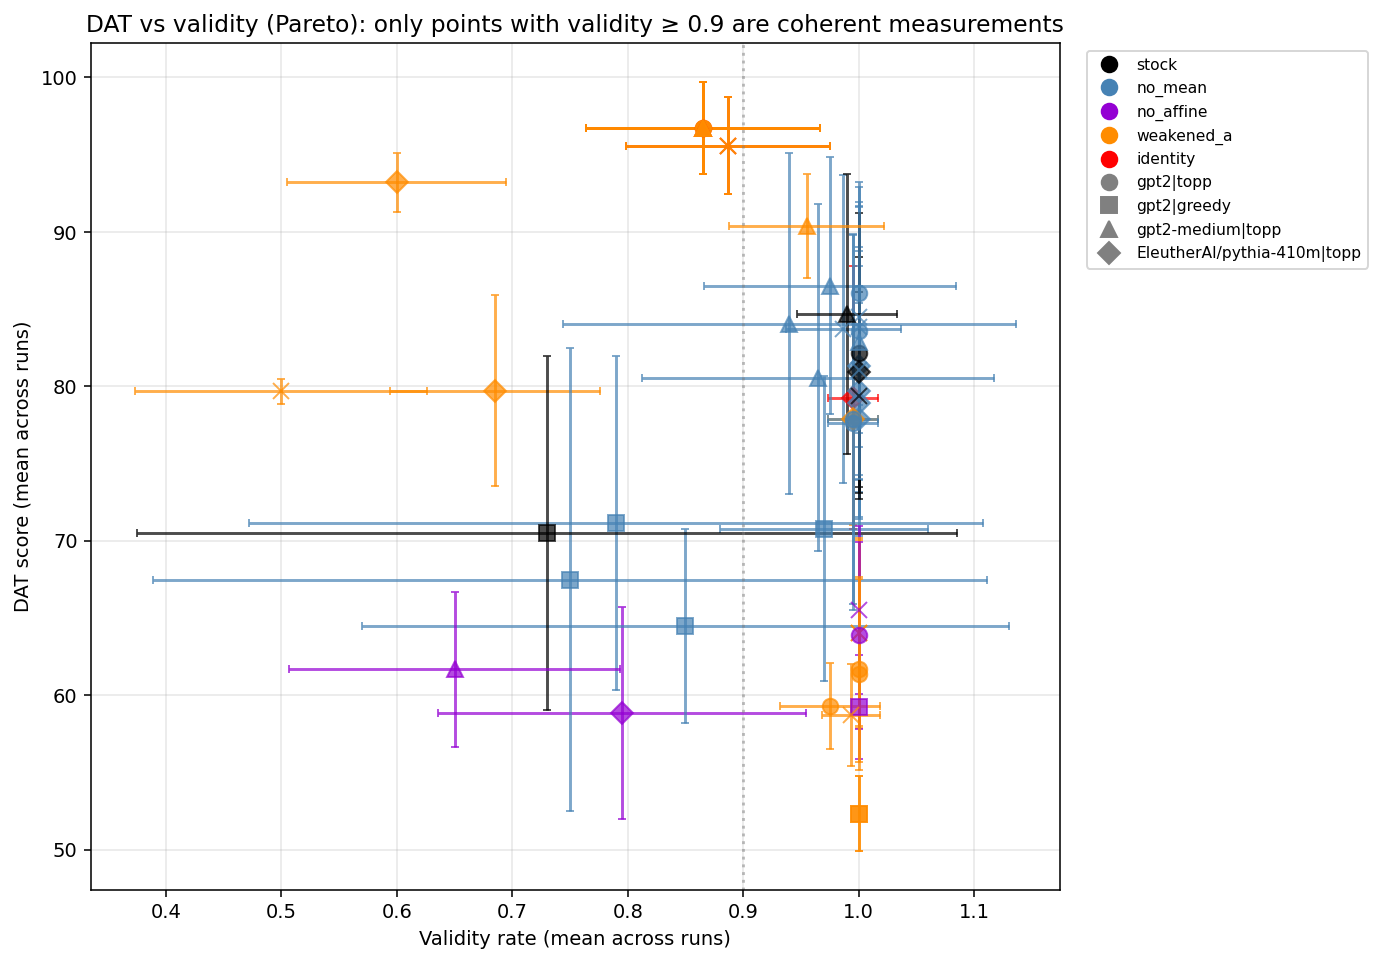
\includegraphics[width=0.95\linewidth]{figures/dat_vs_validity_panel.png}
\caption{\dat versus validity rate across all (model, decoder, intervention)
cells. The cluster at \dat$\approx 96.7$, validity $\approx 0.86$ is the
gibberish ``96.73 trio''. Coherent measurements live in the
validity $\ge 0.9$ band; only those are interpretable as creativity.}
\label{fig:dat-vs-validity}
\end{figure}

\subsection{Per-layer Concept-Association Geometry}
\label{sec:results:geom}

\Figref{fig:geom-layerwise} plots mean pairwise cosine distance among 20
unrelated nouns, layer by layer, for all three models. \tabref{tab:geom}
summarises final-layer pair distance under \nomean.

\begin{figure}[t]
\centering
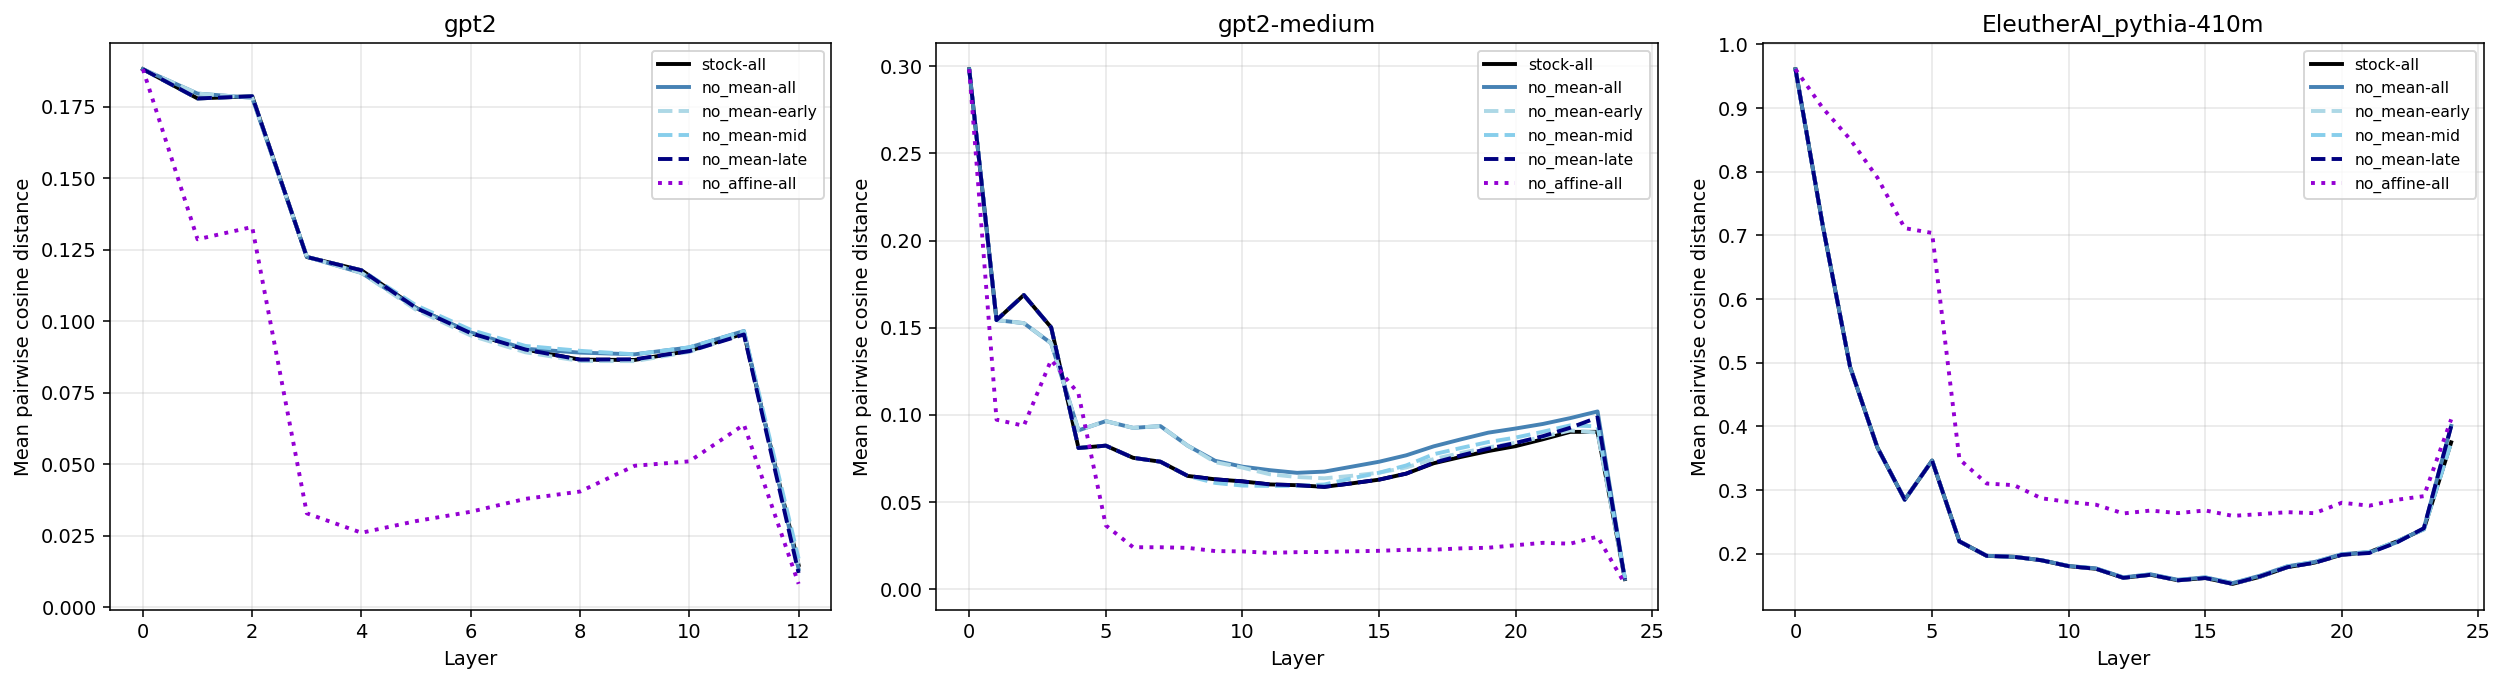
\includegraphics[width=0.95\linewidth]{figures/geometry_layerwise_three_models.png}
\caption{Per-layer mean pairwise cosine distance among 20 unrelated nouns.
Lines show \stockln (solid), \nomean$\,\tgtall$ (dashed), and \nomean$\,$
applied to single layer ranges. \pythia shows the predicted geometric
expansion at the final layer; \gptsmall and \gptmedium do not, because their
final-layer representations are already collapsed into the LM-head mode.}
\label{fig:geom-layerwise}
\end{figure}

\begin{table}[t]
\centering
\caption{Final-layer mean pairwise cosine distance (over 190 noun pairs).
\pythia shows the predicted geometric expansion under \nomean ($+7\%$); the
\gptsmall family does not, because its final-layer representations are
already in a collapsed LM-head mode (pair distance $\sim 0.01$).}
\label{tab:geom}
\begin{tabular}{@{}lllrr@{}}
\toprule
\textbf{Model} & \textbf{Recipe} & \textbf{Target} & \textbf{Pair dist.} & $\Delta$ vs \stockln \\
\midrule
\gptsmall  & \stockln    & --       & 0.0147 & -- \\
\gptsmall  & \nomean     & \tgtall  & 0.0132 & $-0.0014$ ($-9\%$) \\
\gptsmall  & \nomean     & \tgtlate & 0.0119 & $-0.0028$ ($-19\%$) \\
\midrule
\gptmedium & \stockln    & --       & 0.0056 & -- \\
\gptmedium & \nomean     & \tgtall  & 0.0059 & $+0.0002$ ($+4\%$) \\
\gptmedium & \nomean     & \tgtlate & 0.0054 & $-0.0002$ ($-3\%$) \\
\midrule
\pythia    & \stockln    & --       & 0.3749 & -- \\
\pythia    & \textbf{\nomean}     & \textbf{\tgtall}  & \textbf{0.4007} & $\mathbf{+0.0258}$ ($\mathbf{+7\%}$) \\
\pythia    & \noaffine   & \tgtall  & 0.4110 & $+0.0361$ ($+10\%$) \\
\pythia    & \nomean     & \tgtlate & 0.4002 & $+0.0253$ ($+7\%$) \\
\bottomrule
\end{tabular}
\end{table}

Three observations. (i) Only \pythia shows the predicted direction:
removing mean-subtraction expands concept distinguishability by $+7\%$.
The \gptsmall family is already collapsed at the final layer (pair
distance $\sim 0.01$), driven by the residual stream and LM-head geometry,
not by per-block \layernorm. (ii) On \pythia, whole-model and \tgtlate-only
\nomean produce the same $\Delta$; \tgtearly and \tgtmid produce
essentially zero change. The geometric effect is localised to the late
third. (iii) Hidden-state norm grows through the residual stream and is
only pulled back at the final block. \layernorm's per-layer effect is to
\emph{bound} this growth, but in \gptsmall the final-layer compression is
not driven by per-block mean-subtraction.

\subsection{Cross-Modality Reconciliation}
\label{sec:results:reconcile}

\tabref{tab:reconcile} aligns the geometric and behavioural effects of
\nomean side by side. Two patterns emerge.

\begin{table}[t]
\centering
\caption{Effect of removing mean-subtraction (\nomean) across modalities.
The geometric expansion on \pythia ($+7\%$) propagates to \dat only under
high-$T$ decoding on \gptsmall.}
\label{tab:reconcile}
\begin{tabular}{@{}lr@{}}
\toprule
\textbf{Quantity} & \textbf{Effect of \nomean} \\
\midrule
Final-layer concept-pair distance (\pythia)            & $+7\%$ \\
Final-layer concept-pair distance (\gptsmall)          & $-9\%$ \\
Perplexity (\pythia)                                   & $+3\%$ (free) \\
Perplexity (\gptsmall)                                 & $+12\%$ (usable) \\
\dat (\gptsmall + \topp)                                & $+1.8\%$, n.s. \\
\dat (\gptsmall + \greedy)                              & $+0.4\%$, n.s. \\
\dat (\gptmedium + \topp)                               & $-0.7\%$, n.s. \\
\dat (\pythia + \topp)                                 & $-3.8\%$, n.s. \\
\textbf{\dat (\gptsmall + \hight, $T{=}1.2$)}           & $\mathbf{+5.4\%}$, all 4 targets $+$ \\
\bottomrule
\end{tabular}
\end{table}

First, the geometric shift is real but model-specific: it appears at
\pythia's final layer and is absent in \gptsmall's already-collapsed
final layer. Second, the behavioural shift is decoder-specific: at low or
moderate temperature, the freed latent variation does not surface; only at
$T{=}1.2$ does \nomean lift \dat consistently across all four layer
targets. This is consistent with the joint-gating story --- both a wider
latent space \emph{and} a less-sharp decoder are needed to surface
creative outputs. Either alone is insufficient.

\Figref{fig:humans-llms} contextualises the absolute scale: stock-\dat
means for our three models ($70.5, 80.9, 82.1, 84.7$) sit slightly above
the human median ($\sim\!78\!-\!79$) reported by
\citet{olson2021naming}, consistent with \citet{chen2023probing}'s finding
that LLMs already beat the median human on \dat. The \layernorm
interventions we tested do not move models meaningfully relative to the
human distribution.

\begin{figure}[t]
\centering
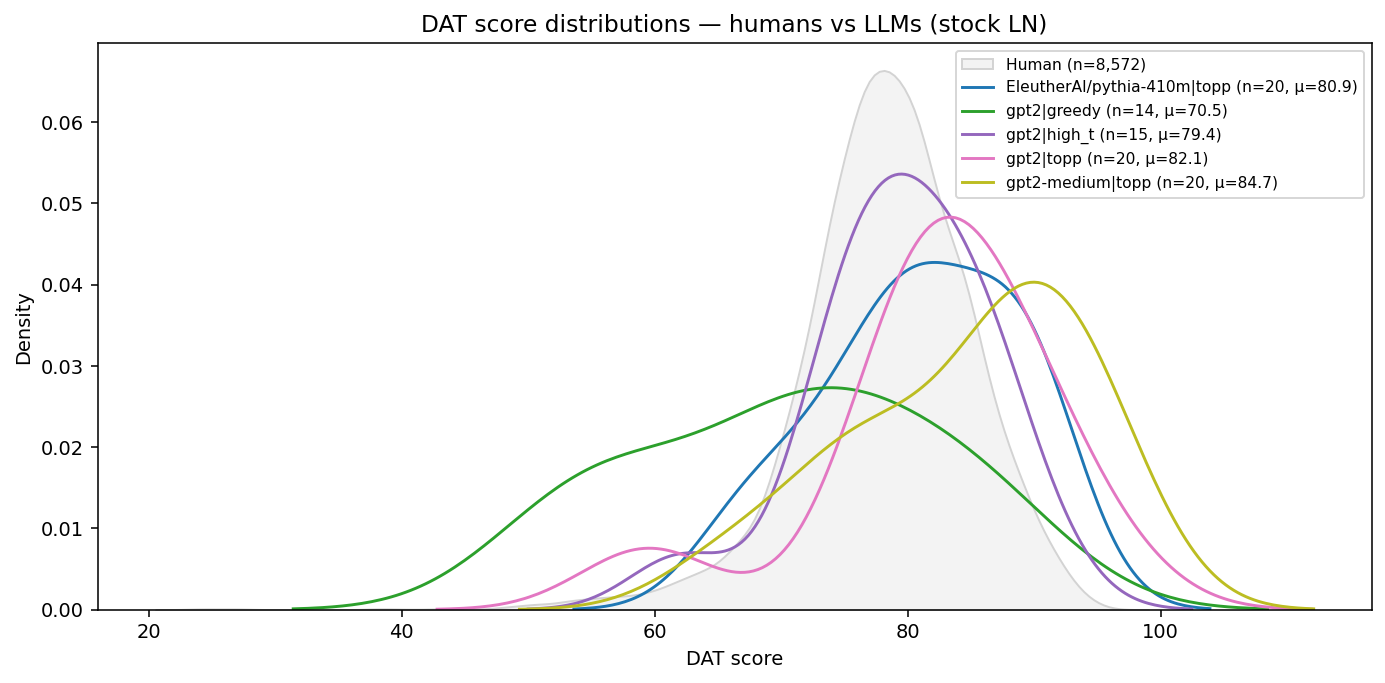
\includegraphics[width=0.7\linewidth]{figures/humans_vs_llms.png}
\caption{Stock-\dat distributions for \gptsmall, \gptmedium, and \pythia
overlaid on the \citet{olson2021naming} human-baseline KDE. All three
models sit slightly above the human median; \layernorm interventions
within the fluency-preserving regime do not displace this position.}
\label{fig:humans-llms}
\end{figure}
